\chapter{波函数、密度矩阵与定域性}

\lectureoverview{贝尔定理之所以被推迟，有一个根本原因：在追问贝尔定理禁止什么之前，我们必须精确说明纠缠是什么。一个双体态是纠缠的，当且仅当它不能分解为属于Alice的一个态与属于Bob的一个态。波函数使这一判据变得具体，关联揭示其后果，而单态则提供了决定性的例子。约化密度矩阵随后成为纠缠整体中某一部分的完整局域描述。有了这套工具，测量表现为一种产生纠缠的相互作用，系统--观察者的边界可以在不改变预言的情况下移动，而纠缠与定域性之间表面上的张力可以被尖锐地陈述出来：遥远的选择改变条件关联，但不改变可用于发送信号的无条件统计量。}

\section{纠缠究竟意味着什么}

人们很容易直接进入贝尔定理。这个定理很美，但它的意义无法与它所检验的结构分开。因此，更紧迫的问题还不是量子力学是否违反贝尔不等式，而是一个纠缠态对复合系统说明了什么。

一个常见的说法是，两个纠缠系统\emph{共享一个态}。这个说法没有区分任何东西。每个复合系统都有一个态，无论纠缠与否。区别在于因式分解。如果\(A\)和\(B\)的希尔伯特空间分别为\(\mathcal H_A\)和\(\mathcal H_B\)，那么这一对系统的态位于
\begin{equation}
\mathcal H_{AB}=\mathcal H_A\otimes\mathcal H_B.
\end{equation}
当一个纯态可以写成
\begin{equation}
\ket{\Psi}_{AB}=\ket{\psi}_A\otimes\ket{\phi}_B.
\label{eq:l7-product-state}
\end{equation}
时，它就是乘积态。如果不存在这样一对因子，那么\(\ket{\Psi}_{AB}\)就是纠缠的。

\begin{classroomqa}
\audiencequestion{纠缠是否仅仅意味着两个系统出现在同一个态矢量中？}
\lecturerresponse{不是。乘积态也属于整个系统的希尔伯特空间。纠缠是更强的、与基无关的陈述：整体的矢量不能写成Alice的一个矢量乘以Bob的一个矢量。}
\end{classroomqa}

\begin{classroomqa}
\audiencequestion{一个巧妙的基变换能否把纠缠态变成乘积态？}
\lecturerresponse{如果基变换是局域的，即对Alice作一种基变换、对Bob作另一种基变换，则不能。局域基变换改变每个因子的坐标，但不改变态是否因式分解。联合希尔伯特空间的完全任意基可以隐藏张量积结构，但它不改变哪些物理自由度属于Alice和Bob。}
\end{classroomqa}

\section{波函数作为希尔伯特空间中的坐标}

\emph{波函数}一词带有历史意象，而这并不是其数学定义的一部分。波函数是态矢量在选定基下的坐标表示。设一组完备的对易可观测量具有共同本征矢量
\begin{equation}
\ket{a,b,c,\ldots}.
\end{equation}
这些标记必须是完备的：合在一起，它们区分基中的每一个矢量。于是
\begin{align}
\ket{\Psi}
&=\sum_{a,b,c,\ldots}
\ket{a,b,c,\ldots}
\braket{a,b,c,\ldots}{\Psi} \\
&=\sum_{a,b,c,\ldots}
\psi(a,b,c,\ldots)\ket{a,b,c,\ldots},
\label{eq:l7-wavefunction-expansion}
\end{align}
其中
\begin{equation}
\psi(a,b,c,\ldots)
=\braket{a,b,c,\ldots}{\Psi}.
\label{eq:l7-wavefunction-definition}
\end{equation}
对于连续标记，相应的求和变为积分。

\begin{figure}[htbp]
\centering
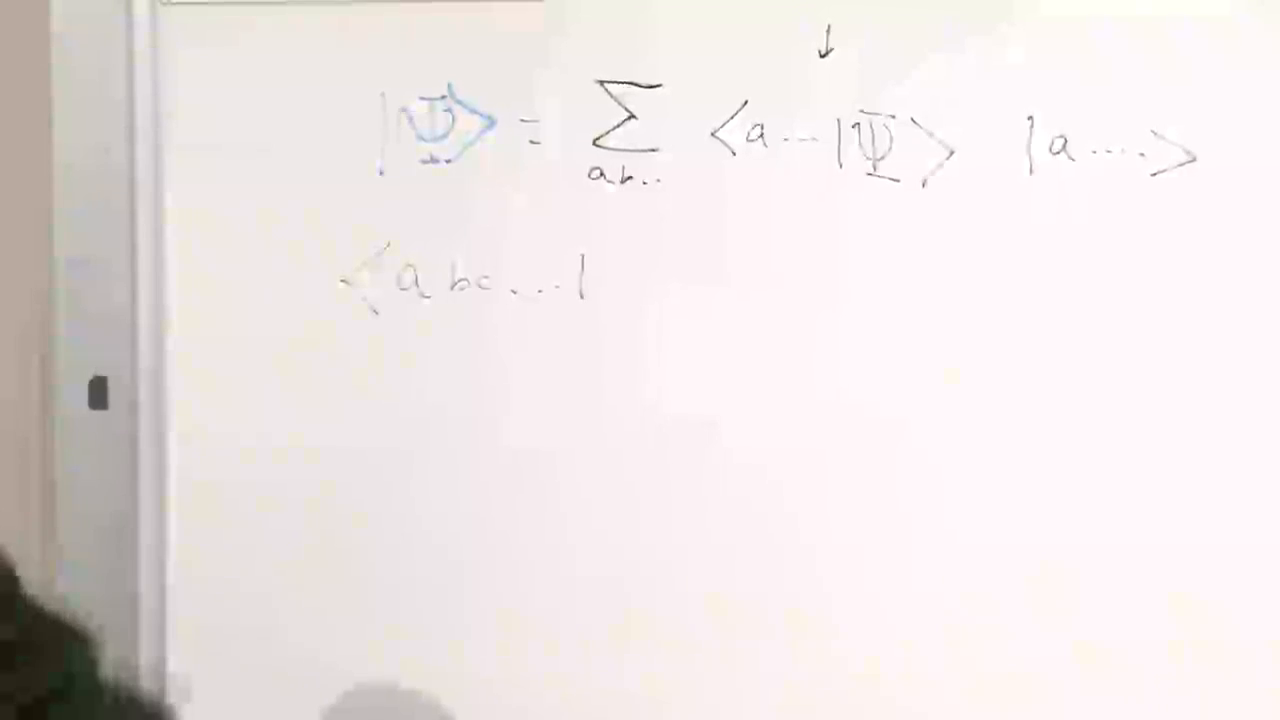
\includegraphics[width=0.88\textwidth]{lecture_07_figure_01.png}
\caption{波函数作为态在完备基下的系数集合。}
\lectureframe{00:07:00}
\end{figure}

对于三维空间中的粒子，对易标记可以是\(x,y,z\)，而
\begin{equation}
\psi(x,y,z)=\braket{x,y,z}{\Psi}
\end{equation}
就是Schr\"odinger熟悉的位形空间波函数。对于\(\sigma_z\)基中的一个自旋，波函数只是这一对
\begin{equation}
\psi(u)=\braket{u}{\Psi},
\qquad
\psi(d)=\braket{d}{\Psi}.
\end{equation}
对于两个自旋，需要两个标记：
\begin{equation}
\Psi(a,b)=\braket{a,b}{\Psi},
\qquad
a,b\in\{u,d\}.
\label{eq:l7-two-spin-wavefunction}
\end{equation}
这个定义中没有任何东西要求空间中存在字面意义上的波。

\begin{classroomqa}
\audiencequestion{改变波函数基是否就是傅里叶变换？}
\lecturerresponse{傅里叶变换是位置表象与动量表象之间的特定基变换。更一般地说，正交归一基的每一种改变都是坐标的幺正变换。从\(\sigma_z\)基到\(\sigma_x\)基的过渡类似于傅里叶变换，尽管它是有限维幺正矩阵，而不是位置--动量积分变换。}
\end{classroomqa}

\begin{classroomqa}
\audiencequestion{如果波函数在基变换下改变，物理态是否也改变了？}
\lecturerresponse{没有。右矢\(\ket{\Psi}\)是抽象态。数\(\psi(a,b,c,\ldots)\)是它在选定基下的坐标。改变坐标会改变这些数，同时使矢量以及所有物理预言保持不变。}
\end{classroomqa}

\section{分量形式的期望值}

在引入密度矩阵之前，先揭示期望值的分量结构。设\(L\)为一个可观测量，其矩阵元为
\begin{equation}
L_{a'a}=\bra{a'}L\ket{a}.
\label{eq:l7-matrix-elements}
\end{equation}
若\(\ket{\Psi}=\sum_a\psi(a)\ket{a}\)，则
\begin{align}
\expect{L}
&=\bra{\Psi}L\ket{\Psi} \\
&=\sum_{a',a}
\psi^*(a')\bra{a'}L\ket{a}\psi(a) \\
&=\sum_{a',a}\psi^*(a')L_{a'a}\psi(a).
\label{eq:l7-expectation-components}
\end{align}

\begin{figure}[htbp]
\centering
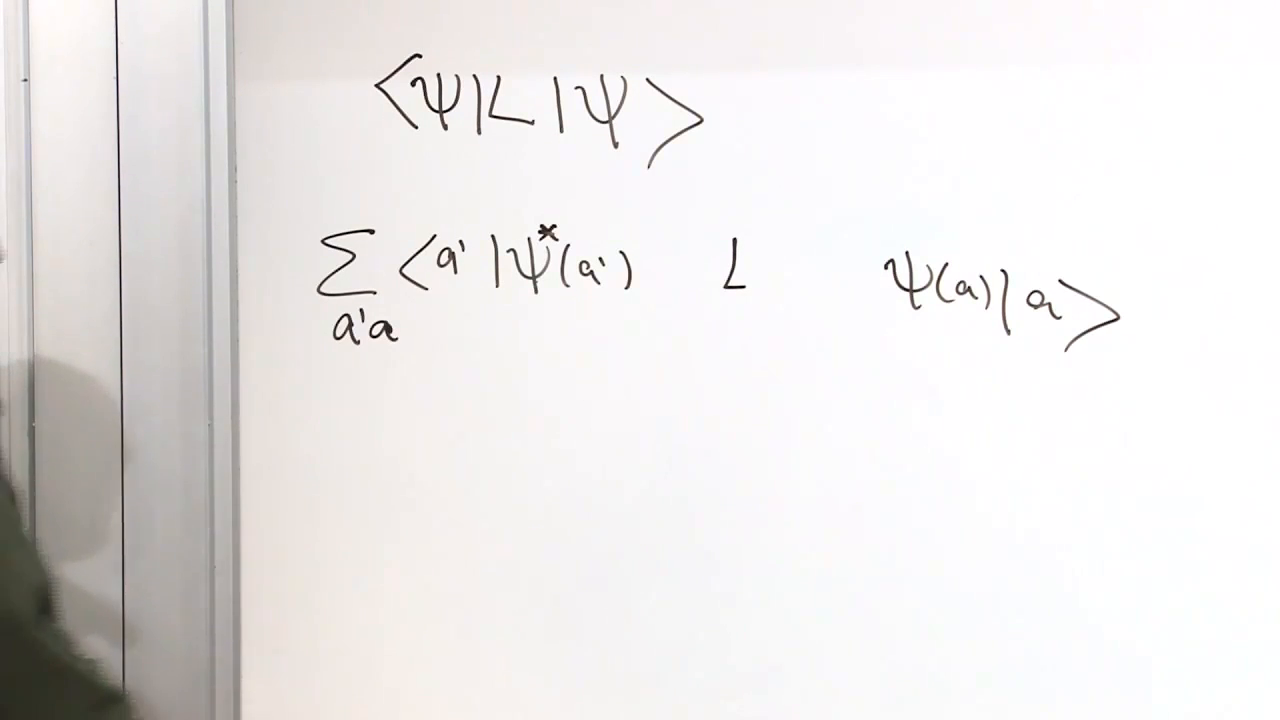
\includegraphics[width=0.88\textwidth]{lecture_07_figure_02.png}
\caption{将期望值的夹心结构展开为波函数系数与矩阵元。}
\lectureframe{00:14:08}
\end{figure}

现在把系统分为Alice的部分和Bob的部分。设\(a\)为Alice的完备基标签，\(b\)为Bob的完备基标签：
\begin{equation}
\ket{\Psi}_{AB}
=\sum_{a,b}\Psi(a,b)\ket{a,b}.
\label{eq:l7-composite-expansion}
\end{equation}
仅属于Alice的可观测量在复合空间上表示为
\begin{equation}
L_A=L\otimes I_B,
\end{equation}
因此其矩阵元为
\begin{equation}
\bra{a',b'}L_A\ket{a,b}
=L_{a'a}\delta_{b'b}.
\label{eq:l7-alice-local-matrix}
\end{equation}
同样，局域于Bob的可观测量具有形式
\begin{equation}
M_B=I_A\otimes M,
\qquad
\bra{a',b'}M_B\ket{a,b}
=\delta_{a'a}M_{b'b}.
\label{eq:l7-bob-local-matrix}
\end{equation}
未受作用因子中的单位算符这一数学表述说明：Alice的操作作用于Alice，Bob的操作作用于Bob。

将式~\eqref{eq:l7-alice-local-matrix}代入期望值，得到
\begin{equation}
\expect{L_A}
=\sum_{a',a,b}
\Psi^*(a',b)L_{a'a}\Psi(a,b).
\label{eq:l7-local-expectation}
\end{equation}
这个公式已经包含了约化密度矩阵；在首先看清因式分解的作用之后，我们将重新整理它。

\begin{classroomqa}
\audiencequestion{为什么式~\eqref{eq:l7-local-expectation}中只剩下一个Bob指标？}
\lecturerresponse{Bob空间上的单位算符贡献了\(\delta_{b'b}\)。它使Bob一侧的bra和ket标签相等，因此对\(b',b\)的双重求和坍缩为对\(b\)的单重求和。}
\end{classroomqa}

\begin{classroomqa}
\audiencequestion{Alice需要知道Bob使用哪个基吗？}
\lecturerresponse{没有任何物理预言依赖于Bob的基。对一个完备的Bob基求和就是单位算符的分解。不同的Bob基会改变各个分量\(\Psi(a,b)\)，但不会改变Alice的期望值。}
\end{classroomqa}

\section{乘积态与关联}

在乘积态中，联合波函数因式分解为：
\begin{equation}
\Psi(a,b)=\psi_A(a)\phi_B(b).
\label{eq:l7-wavefunction-factorization}
\end{equation}
将其代入式~\eqref{eq:l7-local-expectation}：
\begin{align}
\expect{L_A}
&=\sum_{a',a,b}
\psi_A^*(a')\phi_B^*(b)
L_{a'a}
\psi_A(a)\phi_B(b) \\
&=\left[
\sum_{a',a}\psi_A^*(a')L_{a'a}\psi_A(a)
\right]
\left[
\sum_b|\phi_B(b)|^2
\right] \\
&=\bra{\psi_A}L\ket{\psi_A}.
\label{eq:l7-product-local-expectation}
\end{align}
Bob的归一化使其因子等于1。因此Alice拥有与她从未引入Bob系统时完全相同的局域统计。

\begin{figure}[htbp]
\centering
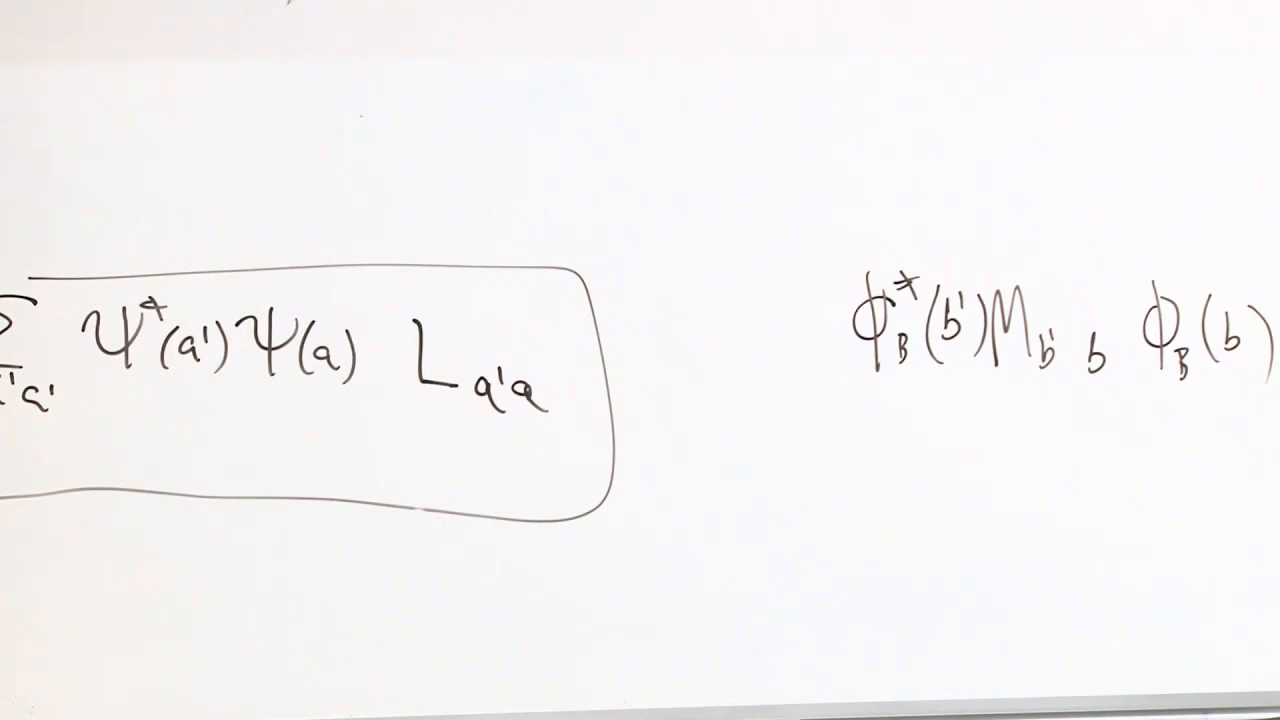
\includegraphics[width=0.88\textwidth]{lecture_07_figure_03.png}
\caption{联合波函数的因式分解以及相应的局域期望值分离。}
\lectureframe{00:29:18}
\end{figure}

一个Alice可观测量与一个Bob可观测量的乘积具有矩阵元
\begin{equation}
\bra{a',b'}L_A M_B\ket{a,b}
=L_{a'a}M_{b'b}.
\end{equation}
对于乘积态，其期望值分离：
\begin{equation}
\expect{L_A M_B}
=\expect{L_A}\expect{M_B}.
\label{eq:l7-product-correlation-factorization}
\end{equation}
因此自然地定义连通关联
\begin{equation}
C(L,M)
=\expect{L_A M_B}
-\expect{L_A}\expect{M_B}.
\label{eq:l7-connected-correlation}
\end{equation}
每个乘积态对每一对局域可观测量都有\(C(L,M)=0\)。反之，对于纯二体态，纠缠保证某一对局域可观测量具有非零连通关联。

\begin{classroomqa}
\audiencequestion{\(L_A M_B\)是否意味着先测量Bob，再测量Alice？}
\lecturerresponse{不是。算符作用于态矢量；仪器执行测量。乘积意味着\(M_B\)作用，然后\(L_A\)作用。由于这些算符占据不同的张量因子，\([L_A,M_B]=0\)，所以它们的数学次序无关紧要。用于估计联合期望值的实验室方案则是另一回事。}
\end{classroomqa}

\begin{classroomqa}
\audiencequestion{即使某个选定的关联为零，态仍可以是纠缠的吗？}
\lecturerresponse{当然可以。一个\(C(L,M)\)为零只说明这一对特定的可观测量不关联。要对纯态确立因式分解，所有局域交叉关联都必须因式分解。部分关联也不必以任何简单的单数值意义意味着部分纠缠；完整的约化密度谱才携带这一信息。}
\end{classroomqa}

\begin{classroomqa}
\audiencequestion{每个关联态都是纠缠的吗？}
\lecturerresponse{对于所讨论的纯态，非因式分解的关联揭示纠缠。对于混合态，普通的经典关联也可以使\(C(L,M)\neq0\)。因此，后来的密度矩阵判据必须附加限定：是否已知整体的态为纯态。}
\end{classroomqa}

\section{单态：整体确定而部分不确定}

设\(\boldsymbol{\sigma}\)作用于Bob的自旋，\(\boldsymbol{\tau}\)作用于Alice的自旋。它们的单态为
\begin{equation}
\ket{S}
=\frac{1}{\sqrt2}
\left(\ket{u d}-\ket{d u}\right),
\label{eq:l7-singlet}
\end{equation}
其中第一个位置是Bob的，第二个是Alice的。两个自旋都没有确定的\(z\)分量：
\begin{equation}
\expect{\sigma_z}=0,
\qquad
\expect{\tau_z}=0.
\label{eq:l7-singlet-local-z}
\end{equation}
然而它们的乘积是确定的：
\begin{equation}
\expect{\sigma_z\tau_z}=-1.
\label{eq:l7-singlet-product-z}
\end{equation}
每一次\(z\)测量都产生相反的结果。

旋转不变性使这一陈述与方向无关。对于任意单位矢量\(\mathbf n\)，
\begin{equation}
\expect{\boldsymbol{\sigma}\cdot\mathbf n}
=\expect{\boldsymbol{\tau}\cdot\mathbf n}=0,
\qquad
\expect{
(\boldsymbol{\sigma}\cdot\mathbf n)
(\boldsymbol{\tau}\cdot\mathbf n)
}=-1.
\label{eq:l7-singlet-any-axis}
\end{equation}
更一般地，
\begin{equation}
\expect{\sigma_i\tau_j}=-\delta_{ij}.
\label{eq:l7-singlet-correlation-tensor}
\end{equation}
每一部分都完全无极化，而沿相同轴的结果则完全反关联。

\begin{figure}[htbp]
\centering
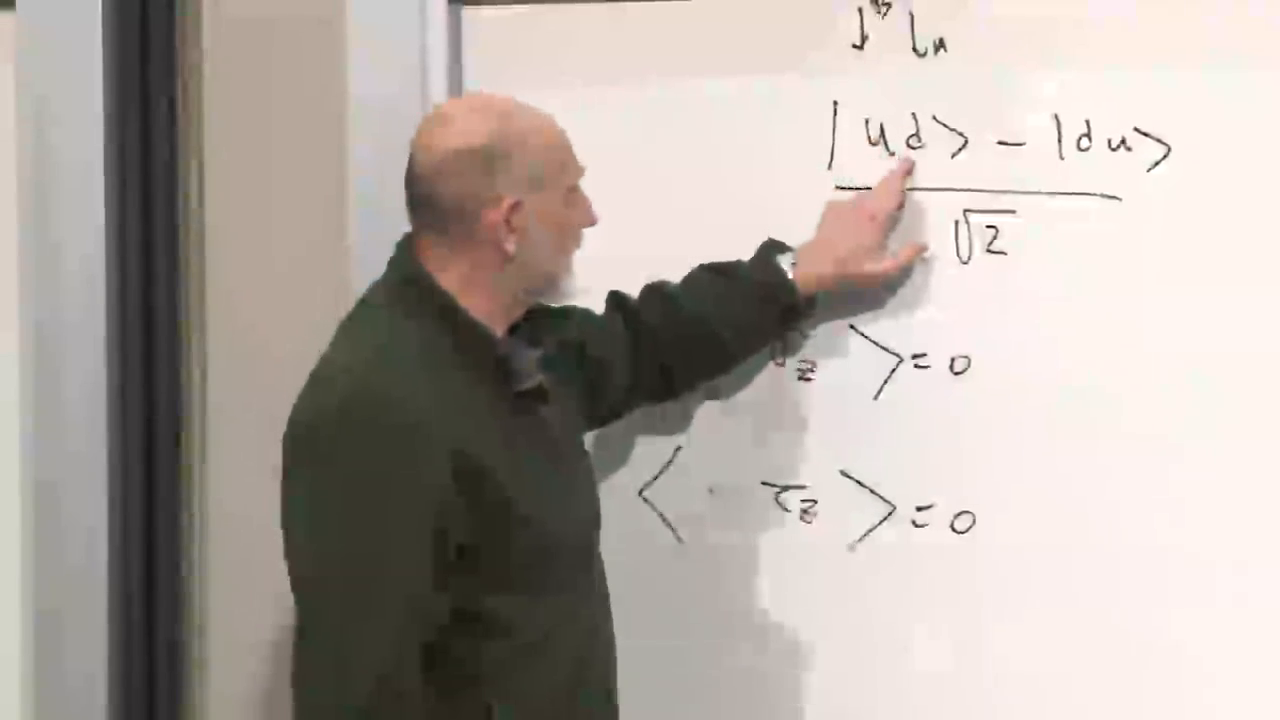
\includegraphics[width=0.88\textwidth]{lecture_07_figure_04.png}
\caption{对于单态，每个局域自旋平均值都为零，而相同分量的乘积为\(-1\)。}
\lectureframe{00:38:28}
\end{figure}

这就是纠缠所产生的特征性反转。对于一个处于纯态中的孤立自旋，存在某个方向，沿该方向其自旋是确定的。而在单态中，没有任何方向能使任一局域自旋成为确定的。尽管如此，复合态仍是纯态，并且被完全指定。关于整体，我们知道了量子力学所允许知道的一切，却仍然无法给其中任何一部分指定一个纯态。

\begin{classroomqa}
\audiencequestion{如果整体的状态已被精确知道，为什么我们不能推断出每个自旋的确定状态？}
\lecturerresponse{因为单态不是乘积态。它的系数不能分解为一个Bob振幅乘以一个Alice振幅。信息存在于各部分之间的关系之中，而不是存在于两个独立存在的局域波函数之中。}
\end{classroomqa}

\begin{classroomqa}
\audiencequestion{像\(\sigma_z\)这样的算符本身是否可能是自旋的一种状态？}
\lecturerresponse{不是。状态是一个矢量，或者更一般地说，是一个密度算符；\(\sigma_z\)是作用于状态上的一个可观测量。\(\sigma_z\)的一个本征矢量是具有确定\(z\)分量的一个状态，但该可观测量与其本征矢量是不同种类的对象。}
\end{classroomqa}

\begin{classroomqa}
\audiencequestion{当我们写出\(\sigma_z\tau_z\ket{S}=-\ket{S}\)时，我们是否已经进行了一次测量？}
\lecturerresponse{没有。该方程记录的是一个算符如何作用于一个矢量。它告诉我们，对相应的联合可观测量的测量必定会返回\(-1\)，但仅仅写出本征值方程并没有把任何探测器包含进来。}
\end{classroomqa}

\begin{classroomqa}
\audiencequestion{一对纠缠粒子能否只是部分关联？}
\lecturerresponse{能。完全反关联是单态在两根轴相等时的一种特殊性质。其他纠缠态可以具有较弱的关联，而且当两根轴不同时，即便是单态给出的也是\(-\mathbf a\cdot\mathbf b\)而不是\(-1\)。纠缠涉及的是不可因子化，而不是在每一次选定的测量中都完全一致或完全不一致。}
\end{classroomqa}

\section{通过能量弛豫制备单态}

旋转不变的双自旋算符
\begin{equation}
\boldsymbol{\sigma}\cdot\boldsymbol{\tau}
=\sigma_x\tau_x+\sigma_y\tau_y+\sigma_z\tau_z
\label{eq:l7-spin-dot-spin}
\end{equation}
组织着四维状态空间。作用于单态时，
\begin{equation}
(\boldsymbol{\sigma}\cdot\boldsymbol{\tau})\ket{S}
=-3\ket{S},
\label{eq:l7-singlet-dot-eigenvalue}
\end{equation}
而三个三重态中的每一个都具有本征值\(+1\)。

\begin{figure}[htbp]
\centering
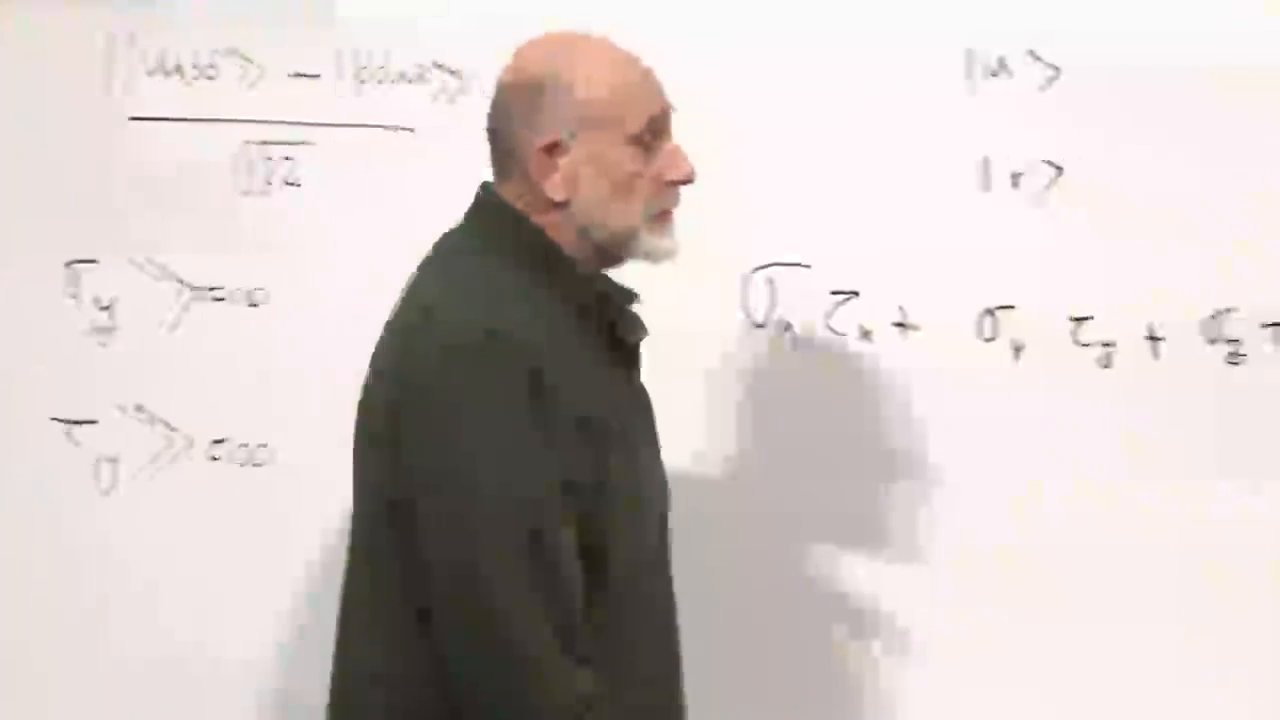
\includegraphics[width=0.88\textwidth]{lecture_07_figure_05.png}
\caption{旋转不变的耦合\(\boldsymbol{\sigma}\cdot\boldsymbol{\tau}\)及其在分离单态与三重态扇区中的作用。}
\lectureframe{00:52:33}
\end{figure}

假设相互作用哈密顿量包含
\begin{equation}
H_{\mathrm{int}}
=J\,\boldsymbol{\sigma}\cdot\boldsymbol{\tau}.
\label{eq:l7-exchange-hamiltonian}
\end{equation}
对于反铁磁耦合\(J>0\)，单态位于三重态之下，低出
\begin{equation}
\Delta E=4J.
\end{equation}
把两个自旋放到一起，让较高能量的成分通过发射一个光子、一个声子或某种其他激发而衰变，于是这对自旋便向单态弛豫。随后可以在保持其联合状态的同时把两个自旋分开，只要这一分离不会引入不受控制的自旋旋转，也不会过于突然地关闭能隙。

同样的能量逻辑也出现在原子系统中。例如在电子偶素中，电子与正电子的自旋耦合把单态与三重态组态分裂开来。通过\(E=mc^2\)，能量差同时也是质量差，尽管光谱学通常把这一分裂报告为能量或频率。

\begin{classroomqa}
\audiencequestion{单态是否总是两个相互作用自旋的基态？}
\lecturerresponse{不是。它是方程~\eqref{eq:l7-exchange-hamiltonian}中符号为\(J>0\)时的基态。把符号反过来会使三重态更低。制备论证依赖于实际的相互作用及其能量排序，而不仅仅依赖于存在两个自旋。}
\end{classroomqa}

\begin{classroomqa}
\audiencequestion{能否通过分别测量全部三个分量来测量\(\boldsymbol{\sigma}\cdot\boldsymbol{\tau}\)？}
\lecturerresponse{不能在一对粒子上通过三次同时的局域自旋测量来做到：\(\sigma_x,\sigma_y,\sigma_z\)互不相容，三个\(\tau\)分量也是如此。它的期望值可以从沿\(x,y,z\)测量的三个子系综重建出来，或者可以通过合适的联合装置直接测量单态--三重态可观测量。}
\end{classroomqa}

\begin{classroomqa}
\audiencequestion{在两个自旋分开之后，它们必须继续相互作用才能保持纠缠吗？}
\lecturerresponse{不必。相互作用是制备或改变状态所需要的，但一旦单态已被制备出来，幺正演化就能保持其纠缠，而无需粒子之间存在持续的力。局域磁场可以使两个因子发生旋转，然而局域幺正旋转本身并不会破坏纠缠。}
\end{classroomqa}

\section{约化密度矩阵}

回到 Alice 的局部期望值：
\begin{equation}
\expect{L_A}
=\sum_{a',a,b}
\Psi^*(a',b)L_{a'a}\Psi(a,b).
\end{equation}
把不属于 \(L\) 的因子重新组合：
\begin{equation}
\expect{L_A}
=\sum_{a',a}
\left[
\sum_b\Psi(a,b)\Psi^*(a',b)
\right]L_{a'a}.
\label{eq:l7-regrouped-expectation}
\end{equation}
方括号中的表达式就是 Alice 的约化密度矩阵，
\begin{equation}
(\rho_A)_{aa'}
=\sum_b\Psi(a,b)\Psi^*(a',b).
\label{eq:l7-reduced-density-components}
\end{equation}
用不依赖基的记号表示，
\begin{equation}
\rho_A
=\operatorname{Tr}_B\ket{\Psi}\bra{\Psi},
\label{eq:l7-partial-trace}
\end{equation}
而每一个 Alice 局部的期望值都是
\begin{equation}
\expect{L_A}
=\operatorname{Tr}_A(\rho_A L).
\label{eq:l7-density-expectation}
\end{equation}

\begin{figure}[htbp]
\centering
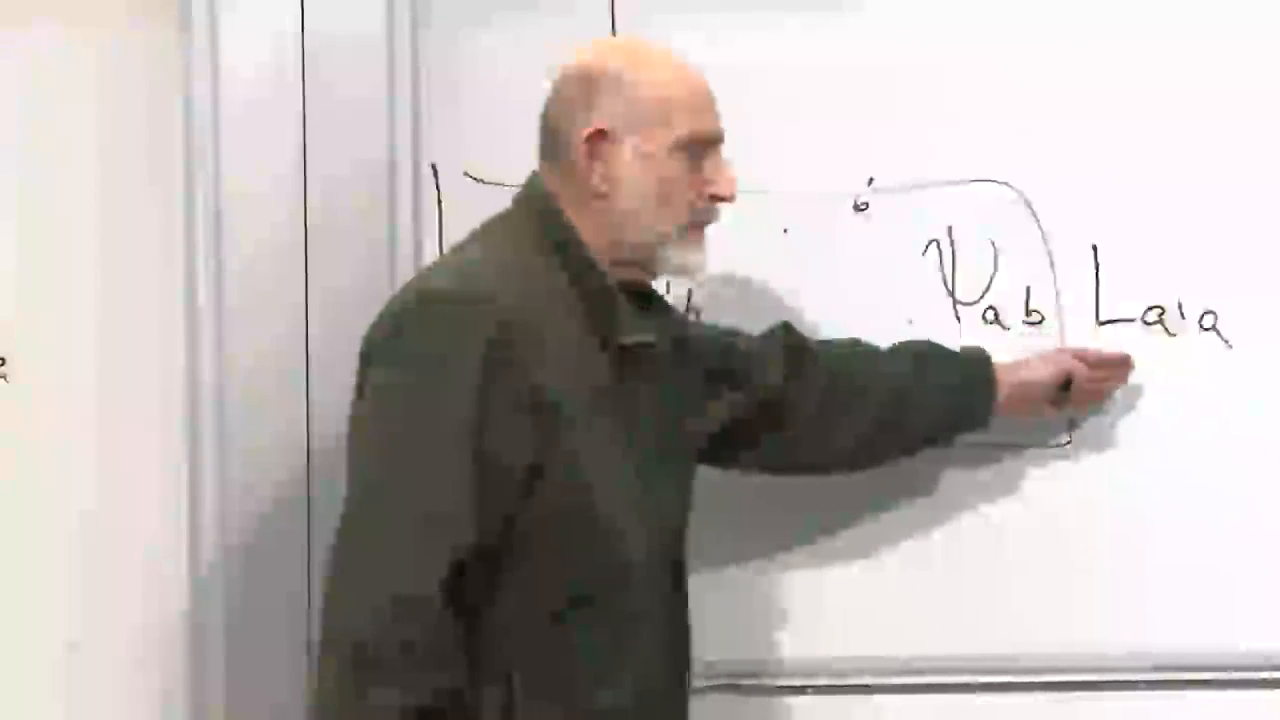
\includegraphics[width=0.88\textwidth]{lecture_07_figure_06.png}
\caption{Alice 的密度矩阵，由对 Bob 的基指标求和联合振幅得到。}
\lectureframe{01:02:33}
\end{figure}

约化密度矩阵是厄米的、正的，并且归一化：
\begin{equation}
\rho_A^\dagger=\rho_A,
\qquad
\bra{\chi}\rho_A\ket{\chi}\geq0,
\qquad
\operatorname{Tr}\rho_A=1.
\label{eq:l7-density-properties}
\end{equation}
它恰好包含局限于 Alice 的所有测量所需的信息。如果两个全局态给出相同的 \(\rho_A\)，那么任何仅涉及 Alice 的实验都无法区分它们。

\begin{classroomqa}
\audiencequestion{Alice 是把密度矩阵作为一个可观测量来测量吗？}
\lecturerresponse{不是在单次测量中。密度矩阵是用来计算所有局部测量概率的对象。给定许多全同制备的系统，Alice 可以通过层析成像重构它：她测量一组足够的可观测量，并从它们的期望值推断出该矩阵。}
\end{classroomqa}

\begin{classroomqa}
\audiencequestion{为什么要对 Bob 求和，而不是选取 Bob 的某一个态？}
\lecturerresponse{因为 Alice 没有来自 Bob 的结果信息。偏迹对 Bob 的一个完备基求和，给出无条件的局部态。若改为选取 Bob 的某一个结果，则会产生一个条件态，这是不同的操作，并且需要知道该结果。}
\end{classroomqa}

对于乘积态 \(\Psi(a,b)=\psi_A(a)\phi_B(b)\)，
\begin{align}
(\rho_A)_{aa'}
&=\sum_b
\psi_A(a)\phi_B(b)
\psi_A^*(a')\phi_B^*(b) \\
&=\psi_A(a)\psi_A^*(a')
\sum_b|\phi_B(b)|^2 \\
&=\psi_A(a)\psi_A^*(a').
\end{align}
因此
\begin{equation}
\rho_A=\ket{\psi_A}\bra{\psi_A}.
\label{eq:l7-pure-projector}
\end{equation}
这是一个秩一投影算符。作用在 \(\ket{\psi_A}\) 上给出
\begin{equation}
\rho_A\ket{\psi_A}
=\ket{\psi_A}\braket{\psi_A}{\psi_A}
=\ket{\psi_A},
\label{eq:l7-density-on-state}
\end{equation}
而对于每一个与 \(\ket{\psi_A}\) 正交的 \(\ket{\chi}\)，
\begin{equation}
\rho_A\ket{\chi}
=\ket{\psi_A}\braket{\psi_A}{\chi}
=0.
\label{eq:l7-density-on-orthogonal}
\end{equation}

\begin{figure}[htbp]
\centering
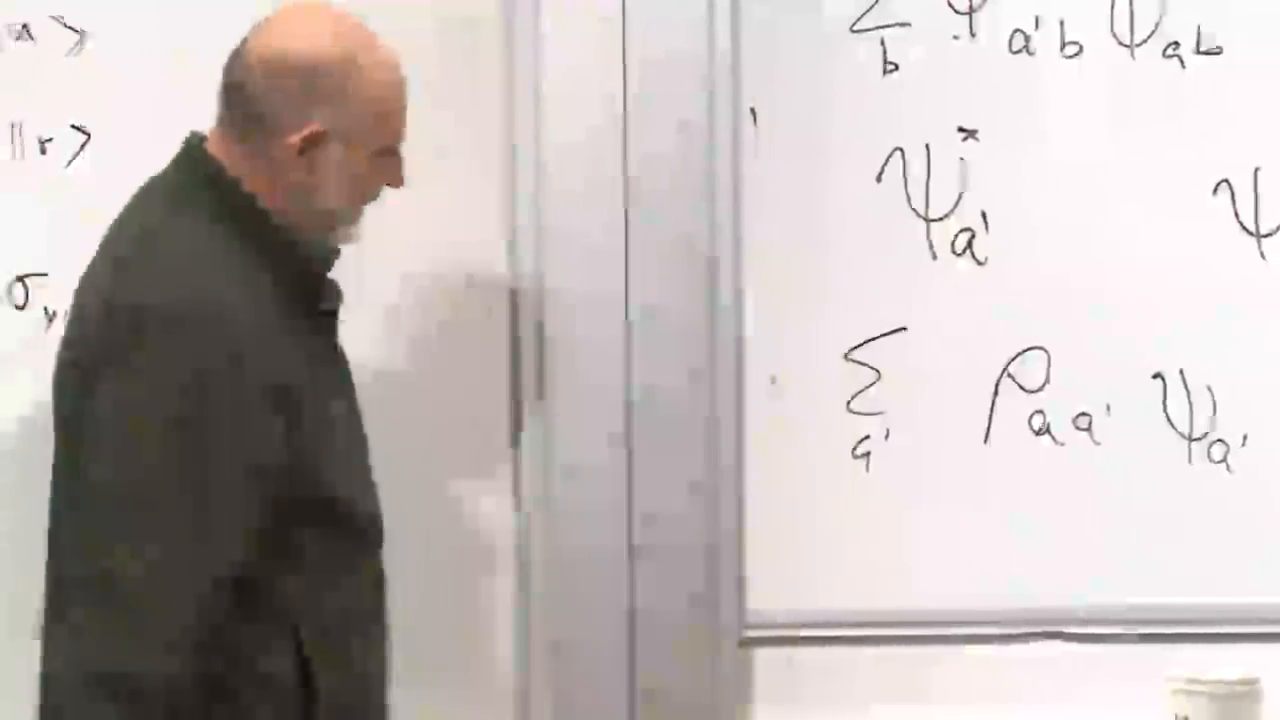
\includegraphics[width=0.88\textwidth]{lecture_07_figure_07.png}
\caption{乘积态的密度矩阵作为投影算符：沿 \(\ket{\psi_A}\) 的本征值为 \(1\)，而在正交矢量上的本征值为 \(0\)。}
\lectureframe{01:09:43}
\end{figure}

\section{密度矩阵谱与纠缠}

\(\rho_A\) 的本征值非负且总和为 1。对于整体的一个纯态：
\begin{itemize}
\item 恰好有一个非零本征值，等于 \(1\)，意味着该态是乘积态；
\item 多于一个非零本征值意味着该态是纠缠的；
\item 在全部可用的局部支集上本征值相等，给出最大纠缠。
\end{itemize}
从施密特分解来看，这一陈述最为清楚，
\begin{equation}
\begin{aligned}
\ket{\Psi}_{AB}
&=\sum_{r=1}^{R}\sqrt{\lambda_r}
\ket{r}_A\ket{r}_B,\\
\lambda_r&\geq0,
\qquad
\sum_r\lambda_r=1.
\end{aligned}
\label{eq:l7-schmidt}
\end{equation}
对此有
\begin{equation}
\rho_A=\sum_{r=1}^{R}\lambda_r\ket{r}_A\bra{r}.
\label{eq:l7-schmidt-density}
\end{equation}
施密特秩 \(R\) 对于乘积态为 1，而对于纠缠纯态则大于 1。

对于单态，
\begin{equation}
\rho_A
=\operatorname{Tr}_B\ket{S}\bra{S}
=\frac12\ket{u}\bra{u}
+\frac12\ket{d}\bra{d}
=\frac12 I.
\label{eq:l7-singlet-reduced-density}
\end{equation}
它的本征值为
\begin{equation}
\operatorname{spec}(\rho_A)
=\left\{\frac12,\frac12\right\}.
\end{equation}
尽管这一对粒子的态是纯态，Alice 的局部态却是最大混合的。

该谱提示了一个定量度量。冯·诺依曼熵
\begin{equation}
S(\rho_A)
=-\operatorname{Tr}(\rho_A\log\rho_A)
=-\sum_r\lambda_r\log\lambda_r
\label{eq:l7-entanglement-entropy}
\end{equation}
对于乘积纯态为零，而当 \(d_A\leq d_B\) 时，对于最大纠缠态达到 \(\log d_A\)。熵的详细用法可以推迟；该谱已经提供了本质的区分。

\begin{classroomqa}
\audiencequestion{纠缠的约化密度矩阵的每一个本征值都必须非零吗？}
\lecturerresponse{不。多于一个非零本征值就足够了。如果 Alice 的空间很大，一个纠缠态可能只占据一个较低维的施密特子空间，从而留下额外的零本征值。最大纠缠意味着在整个较小的子系统上本征值相等，而不仅仅是在任意选取的一个子集上相等。}
\end{classroomqa}

\begin{classroomqa}
\audiencequestion{一个混合的约化密度矩阵本身就能证明 Alice 与 Bob 纠缠吗？}
\lecturerresponse{只有当已知全局态是纯态时才行。混合的局部态也可以由混合全局态中的普通经典混合产生。然而，对于纯的二体态，局部混合性恰好等价于跨该二分割的纠缠。}
\end{classroomqa}

\begin{classroomqa}
\audiencequestion{Alice 的可观测量的所有矩能确定她的概率分布吗？}
\lecturerresponse{在有限维系统中，一个算符基的期望值确定 \(\rho_A\)，而 \(\rho_A\) 通过玻恩定则确定每一个局部结果分布。重构需要一系综全同制备的副本；单个孤立事件无法揭示密度矩阵。}
\end{classroomqa}

\section{作为纠缠相互作用的测量}

把 Alice 和 Bob 替换为一个自旋和一个测量装置。设该装置有一个准备态 \(\ket{0}_D\) 和一个触发态 \(\ket{1}_D\)。一个记录自旋是否向上的理想相互作用可以表示为
\begin{align}
\ket{u}\ket{0}_D&\longrightarrow\ket{u}\ket{1}_D,\\
\ket{d}\ket{0}_D&\longrightarrow\ket{d}\ket{0}_D.
\label{eq:l7-measurement-basis-map}
\end{align}
探测器必须从已知的准备态开始；否则它的末态将无法提供明确的记录。

线性性决定了叠加态的演化：
\begin{equation}
\left(\alpha\ket{u}+\beta\ket{d}\right)\ket{0}_D
\longrightarrow
\alpha\ket{u}\ket{1}_D
+\beta\ket{d}\ket{0}_D.
\label{eq:l7-measurement-entanglement}
\end{equation}
除非某个系数为零，否则末态是纠缠的。仪器之所以获得了信息，正是因为其指针态与自旋相关联。

\begin{figure}[htbp]
\centering
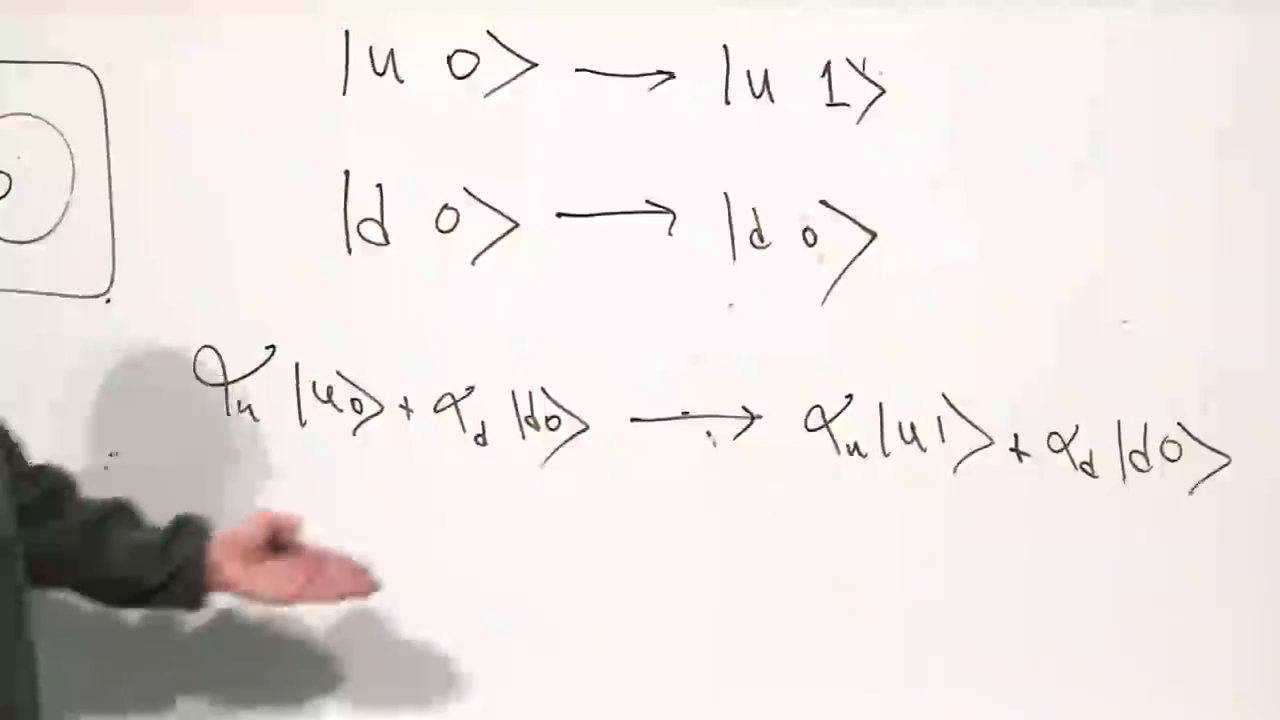
\includegraphics[width=0.88\textwidth]{lecture_07_figure_08.png}
\caption{理想测量将自旋的各备选情形与不同的指针态关联起来，从而产生纠缠。}
\lectureframe{01:20:20}
\end{figure}

如果只保留自旋而忽略探测器，其约化态为
\begin{equation}
\rho_{\mathrm{spin}}
=|\alpha|^2\ket{u}\bra{u}
+|\beta|^2\ket{d}\bra{d},
\label{eq:l7-postmeasurement-reduced-state}
\end{equation}
这里假设指针记录是正交的。干涉项已从局域描述中消失，因为它们被存储在与仪器之间的关联中。

现在有两种互补的描述。如果读取探测器结果并依据记录进行条件化，则自旋被赋予相应的分支：触发后为\(\ket{u}\)，未触发后为\(\ket{d}\)。这就是坍缩描述。如果把探测器和自旋视为一个封闭系统，则方程~\eqref{eq:l7-measurement-entanglement}是普通的幺正演化，没有任何分支从联合态中被移除。

\begin{classroomqa}
\audiencequestion{测量是超越纠缠的某种东西吗？}
\lecturerresponse{在系统--仪器动力学的层面上，测量是一种建立可靠关联的相互作用。坍缩是在选定确定记录之后所使用的条件描述。究竟把这种更新视为基本的，还是视为相对于某个所选割线的，是一个解释性问题；操作层面的预言是一致的。}
\end{classroomqa}

\begin{classroomqa}
\audiencequestion{为什么理想测量使自旋本征态保持不变？}
\lecturerresponse{这就是该模型的可重复性要求。如果输入已经是所测可观测量的本征态，仪器应当记录其值而不改变该值。真实测量可以是破坏性的，但那样一来其相互作用就必须以不同方式建模。}
\end{classroomqa}

\section{观察者层级}

一旦承认仪器是量子系统，就没有自然的理由停在那里。来自指针的光与眼睛相互作用；来自眼睛的信号与大脑相关联；一个观察者可能被另一个观察者观察。Schr\"odinger的猫和维格纳的朋友戏剧化了同样的嵌套结构：
\begin{equation}
\begin{gathered}
\text{spin}
\longrightarrow
\text{apparatus}
\longrightarrow
\text{cat}\\
\longrightarrow
\text{Schr\"odinger}
\longrightarrow
\text{Wigner}.
\end{gathered}
\label{eq:l7-observer-chain}
\end{equation}
在任何选定的边界之内，人们可以用幺正演化和不断增加的纠缠来描述这条链。在边界之外，人们使用以结果条件化的坍缩语言。

关键的相容性条件是边界可以移动。如果猫记录了自旋向上，那么Schr\"odinger后来必须记录一只看到自旋向上的猫，而维格纳必须记录Schr\"odinger记录了同一段历史。量子力学并未指出一条唯一的明确界线，规定客观事件必须在何处被宣告。猫、眼睛和大脑都由物理自由度构成；将其中任何一个豁免于量子力学之外，都需要一条额外的定律。

费曼对由此产生的不适采取务实的态度。概念上的问题可能如此之大，以至于甚至难以陈述是否存在这样一个问题，而计算规则继续预言它们所适用的一切实验。形式体系的目的不是强加某一种解释，而是使不适的来源变得精确：关于整体的完备知识可以与对其任何部分都不存在纯态描述共存。

\begin{classroomqa}
\audiencequestion{如果我是那只猫，我必须在自身处划下界线吗？}
\lecturerresponse{对于你所拥有的确定记录，你可以使用坍缩描述。另一个把你包含在更大孤立系统中的观察者，可以使用纠缠态描述。要求并不是每个人都划下同一条界线，而是当观察者后来比较结果时，所有描述都给出相容的记录。}
\end{classroomqa}

\begin{classroomqa}
\audiencequestion{客观事件发生在哪里：在原子处、猫处、Schr\"odinger处，还是维格纳处？}
\lecturerresponse{幺正形式体系并未选择这些位置中的某一个作为特权边界。也许像\emph{发生}这样的日常词语正被推到其精确性所适用的语境之外。形式工具告诉我们关联如何传播，以及每个观察者能预言什么；决定如何解释最终的边界则是另一项任务。}
\end{classroomqa}

\subsection{弱耦合与不完美读出}

方程~\eqref{eq:l7-measurement-basis-map}中的理想映射产生完全可区分的记录。较弱的相互作用可能使仪器态仅部分可区分：
\begin{equation}
\alpha\ket{u}\ket{D_u}
+\beta\ket{d}\ket{D_d},
\qquad
0<|\braket{D_d}{D_u}|<1.
\label{eq:l7-weak-measurement}
\end{equation}
于是仪器只接收到部分信息，纠缠也不完整。这就是弱测量或非锐测量的情形。

这种情况必须与下游读出不良区分开来。探测器可能已经与自旋完全关联，而眼睛、电缆、放大器或大脑未能清晰地传递记录。在第一种情况下，系统--探测器的相互作用是弱的；在第二种情况下，探测器处存在良好的记录，但后续的信息传递效率低下。探测器效率可能涉及这两个阶段中的任何一个，因此在判定原因之前，必须确定物理耦合。

\begin{classroomqa}
\audiencequestion{如果视力不佳使指针不确定，那么量子测量是弱的吗？}
\lecturerresponse{不一定。自旋可能已经与仪器强烈且完全地关联，而仪器到眼睛或眼睛到大脑的通道却是差的。真正弱的测量意味着初始的系统--仪器耦合本身只产生了部分可区分的记录。}
\end{classroomqa}

\section{定域性与不可传信}

应当赋予\emph{超距作用}这一说法一个操作性的含义。在通常的物理学中，一个远处的动作会改变在这里能够观测到的结果。如果太阳消失了，地球的运动立即改变，而不是在光传播时间之后才改变，那么人们就可以利用这一变化以超光速传递信息。那将是真正的非定域传信。

纠缠不允许这样的传信。设Bob执行一个由Kraus算符\(K_\mu\)表示的局域量子操作，其中
\begin{equation}
\sum_\mu K_\mu^\dagger K_\mu=I_B.
\end{equation}
如果Alice不知道Bob的结果，最终的联合态为
\begin{equation}
\rho'_{AB}
=\sum_\mu
(I_A\otimes K_\mu)\rho_{AB}
(I_A\otimes K_\mu^\dagger).
\end{equation}
对Bob取偏迹得到
\begin{equation}
\rho'_A
=\operatorname{Tr}_B\rho'_{AB}
=\operatorname{Tr}_B\rho_{AB}
=\rho_A.
\label{eq:l7-no-signaling}
\end{equation}
因此，每一个无条件的Alice局域概率都不会因Bob选择保迹的局域操作而改变。

条件态则不同。如果Bob进行测量并得到结果\(\mu\)，Alice可以赋予
\begin{equation}
\rho_{A|\mu}
=\frac{
\operatorname{Tr}_B\!\left[
(I_A\otimes K_\mu)\rho_{AB}
(I_A\otimes K_\mu^\dagger)
\right]
}{p_\mu}.
\label{eq:l7-conditioned-state}
\end{equation}
但Alice无法知道哪一个\(\rho_{A|\mu}\)适用，直到Bob通过普通信号告知\(\mu\)。在消息到达之前，她必须对所有结果取平均：
\begin{equation}
\sum_\mu p_\mu\rho_{A|\mu}=\rho_A.
\label{eq:l7-conditioned-average}
\end{equation}

\begin{classroomqa}
\audiencequestion{如果Bob先测量，Alice的密度矩阵何时改变？}
\lecturerresponse{她的无条件密度矩阵不会改变。一旦Bob的结果到达她那里，她可以用相应的条件密度矩阵来替换它。这一更新反映了新获得的信息，并且在经典消息到达之前不能使用。}
\end{classroomqa}

\begin{classroomqa}
\audiencequestion{Bob的测量是否在同一瞬间物理地坍缩了Alice的态？}
\lecturerresponse{不同的诠释对条件更新的描述不同，但都同意可检验的陈述：Alice的局域结果概率保持不变，直到来自Bob的信息变得可用。不会产生任何可控的瞬时信号。}
\end{classroomqa}

设想许多单态对分布在编号的行中。Bob对其中一个成员测量\(z\)，对另一个测量\(x\)，对再一个测量\(y\)，依此类推。Alice的局域结果对每一行都保持为无偏序列：
\begin{equation}
P_A(+|\mathbf a)=P_A(-|\mathbf a)=\frac12.
\label{eq:l7-alice-marginal}
\end{equation}
她的记录中没有任何东西揭示Bob选择了哪些轴或得到了哪些结果。

\begin{figure}[htbp]
\centering
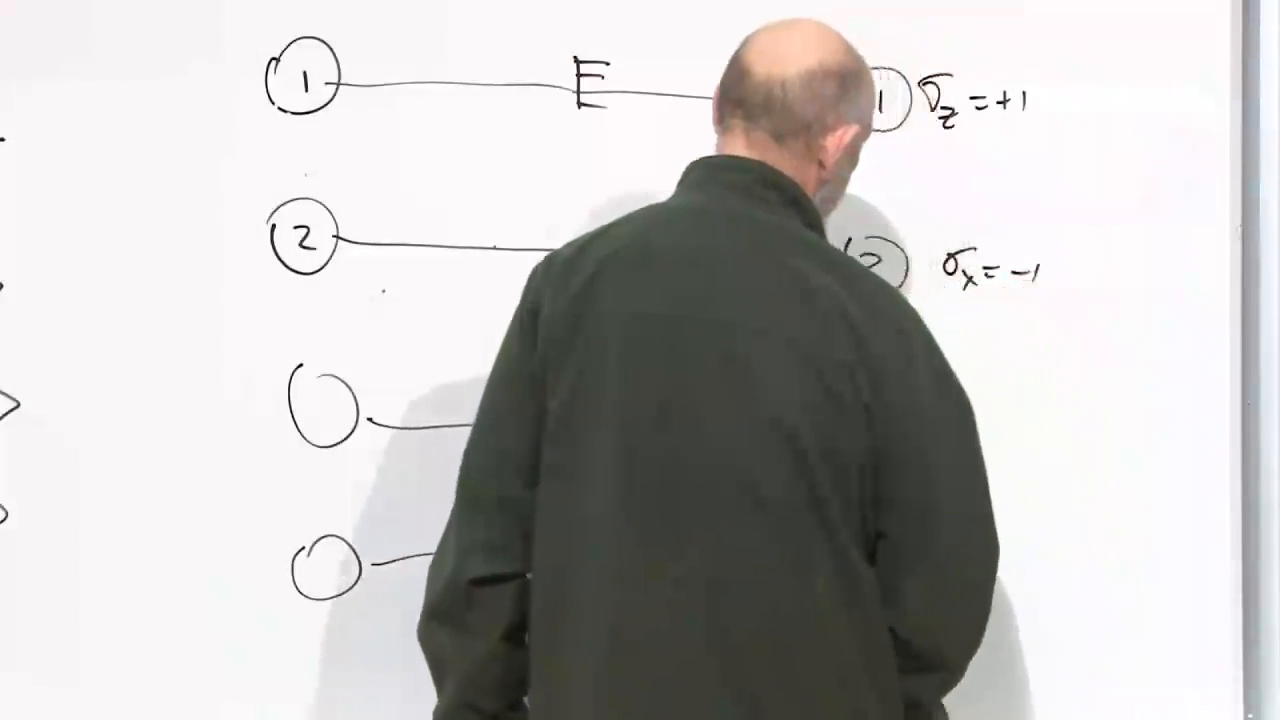
\includegraphics[width=0.88\textwidth]{lecture_07_figure_09.png}
\caption{许多独立制备的粒子对允许将不同的测量轴分配给不同的行；Alice的边缘统计保持不变。}
\lectureframe{01:49:00}
\end{figure}

在受光速限制的电报到达并列出每一行Bob的轴和结果之后，Alice可以整理她的记录。同轴单态测量随后将逐对呈现相反的结果。该消息揭示了联合统计中已经存在的关联；它不会追溯性地改变Alice先前的局域频率分布。

\begin{classroomqa}
\audiencequestion{Alice能否从她自己数据的足够多阶矩中推断出Bob的选择？}
\lecturerresponse{不能。所有Alice局域矩都由\(\rho_A\)固定，而方程~\eqref{eq:l7-no-signaling}使该矩阵保持不变。更多的副本会改善她对同一局域密度矩阵的估计；它们不会揭示Bob的基或结果。}
\end{classroomqa}

\begin{classroomqa}
\audiencequestion{如果Bob对系综的每一个成员都选择不同的轴呢？}
\lecturerresponse{Alice仍然看到相同的局域分布。一旦Bob发送逐行的设置和结果，双方就可以比较每一对轴的条件关联。设置依赖性出现在联合统计中，而不是Alice的边缘统计中。}
\end{classroomqa}

\section{作为模拟博弈的Bell问题}

无信号传递与贝尔非定域性之间的区别，在经典模拟这一问题中变得更加清晰。从一个自旋开始，
\begin{equation}
\ket{\psi}=\alpha_u\ket{u}+\alpha_d\ket{d},
\qquad
|\alpha_u|^2+|\alpha_d|^2=1.
\end{equation}
经典程序可以存储两个复振幅，用Schr\"odinger方程演化它们，并接受用户选定的测量方向。当发出测量命令时，程序计算玻恩概率，使用伪随机数发生器选择一个结果，显示该结果，并将其存储的状态更新为相应的本征态。重复这一过程即可再现单个自旋的统计规律。

因此，仅凭随机性并不能划出经典力学与量子力学之间的分界线。经典计算机能够生成在操作意义上足够随机、足以用于模拟的序列，即使其伪随机算法在底层是确定性的。

对于处于乘积态的两个自旋，两台分离的计算机也足够了。Alice的计算机存储并演化\(\ket{\psi_A}\)；Bob的存储并演化\(\ket{\phi_B}\)。每一台只响应其本地设置。由于联合概率因子化，计算机分离之后不需要任何通信。

纠缠对改变了问题。人们可以在实验之前把两台机器放在一起，装入关联的隐变量数据，同步它们的时钟，甚至给它们相同的随机种子。然而在分离之后，每个输出必须只依赖于其本地测量设置以及事先提供的共享信息。贝尔定理表明，对于自由选择的设置，没有任何这样的定域隐变量方案能够再现全部量子关联。

\begin{figure}[htbp]
\centering
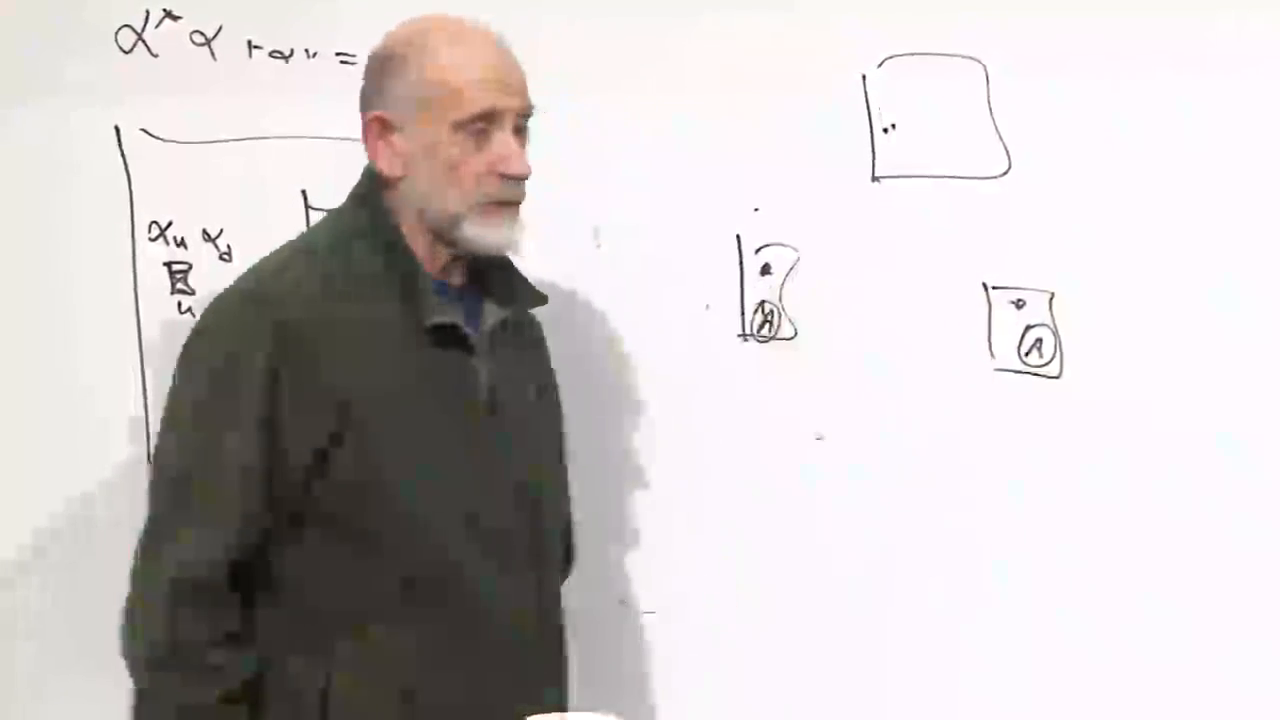
\includegraphics[width=0.88\textwidth]{lecture_07_figure_10.png}
\caption{分离计算机模型：本地程序可以共享制备数据，但分离之后它们不能交流测量设置。}
\lectureframe{02:00:00}
\end{figure}

如果计算机之间保留连线，使得设置和结果可以交换，那么模拟就能再现这些关联。但这样一来，这一对就不再是真正分离的定域模型；它作为一台连通的计算机运作。障碍并不在于抽象意义上的经典计算。单台全局经典机器可以通过存储完整的联合波函数来模拟有限量子系统，尽管所需内存一般随子系统数目指数增长。贝尔的障碍针对的是分解为独立运作的本地机器。

\begin{classroomqa}
\audiencequestion{为什么两台计算机不能简单地使用同一个随机数序列？}
\lecturerresponse{共享随机性在定域隐变量模型中本来就是允许的。它可以预先确定关联的答案，但每个答案必须对该侧后来可能选择的每一个测量设置都成立。贝尔不等式表达了所有这类预先安排的定域策略所服从的约束；量子关联违反这些约束。}
\end{classroomqa}

\begin{classroomqa}
\audiencequestion{随机数必须依赖于测量方向吗？}
\lecturerresponse{本地输出可以依赖于它自己的本地方向和共享的隐变量数据，但不能依赖于分离之后所选择的远处方向。允许依赖于两个设置就需要通信、逆因果性，或者通常的测量独立性假设失效。贝尔定理使这些假设变得明确，而不是把它们隐藏在\emph{随机}这个词里。}
\end{classroomqa}

\begin{classroomqa}
\audiencequestion{两台分离的量子计算机能否在经典程序失败的地方取得成功？}
\lecturerresponse{如果它们共享纠缠的量子自由度，就能成功。在这种情况下，计算机并不是用本地经典记录来模拟纠缠；它们在物理上拥有纠缠。它们的本地结果仍然不能传递可控的超光速信息。}
\end{classroomqa}

\begin{classroomqa}
\audiencequestion{一台普通的经典计算机能否模拟整个纠缠对？}
\lecturerresponse{可以。它可以在一个地方存储四个联合振幅并计算所有测量概率。对于许多粒子，这种直接模拟会变得昂贵，因为希尔伯特空间维数指数增长，但当所有信息都在一台机器内部全局可用时，并不存在贝尔矛盾。}
\end{classroomqa}

\begin{classroomqa}
\audiencequestion{那么贝尔定理是否证明了通常意义上的超距作用？}
\lecturerresponse{它证明的是，满足贝尔假设的定域隐变量解释无法再现观测到的关联。它并没有为Alice或Bob提供超光速信号传递通道。贝尔非定域性与操作意义上的超光速通信是不同的主张。}
\end{classroomqa}

\section{本地能学到什么？}

局域可观测量与联合可观测量不可混为一谈。Bob 可以测量 \(\sigma_x\)，Alice 可以测量 \(\tau_x\)；通过事后比较记录，他们估计
\begin{equation}
\expect{\sigma_x\tau_x}.
\end{equation}
单独的局域装置都不能测量该乘积。转动标量
\begin{equation}
\boldsymbol{\sigma}\cdot\boldsymbol{\tau}
=\sigma_x\tau_x+\sigma_y\tau_y+\sigma_z\tau_z
\end{equation}
要么需要针对三项的不同子系综，要么需要一台能分辨单态和三重态扇区的新型联合装置。利用原来的局域自旋测量仪，无法从一对粒子获得全部三个互不相容的分量乘积。

\begin{classroomqa}
\audiencequestion{是否存在整体的可观测量，是 Alice 和 Bob 原来的装置无法分别测量的？}
\lecturerresponse{是的。像 \(\sigma_x\tau_x\) 这样的单个乘积，可以通过两次局域 \(x\) 测量再加以比较来估计。和 \(\boldsymbol{\sigma}\cdot\boldsymbol{\tau}\) 无法由对一对粒子的同时 \(x,y,z\) 读数拼装出来。它需要一次真正的联合单态--三重态测量，或者针对互不相容各项的独立系综。}
\end{classroomqa}

Bob 无法从单次事件推断纠缠。然而，对于许多相同制备的副本，他可以重构自己的约化密度矩阵。对于量子比特，
\begin{equation}
\rho_B
=\frac12\left(
I+\mathbf r\cdot\boldsymbol{\sigma}
\right),
\label{eq:l7-bloch-density}
\end{equation}
而沿若干轴的测量确定布洛赫矢量 \(\mathbf r\)。若 \(|\mathbf r|=1\)，则 Bob 的局域态是纯态；若 \(|\mathbf r|<1\)，则它是混合态。在已知每次试验的全局制备都是同一纯态的特殊情形下，局域混合性证明 Bob 与他的子系统之外的某物纠缠。

对于两个纯自旋的乘积态，Bob 可以寻找极化方向 \(\mathbf n=\mathbf r/|\mathbf r|\)。沿该轴重复测量会返回一个确定答案。对于单态，\(\mathbf r=0\)，因此每个轴在局域上仍保持随机。这种寻找永远找不到极化方向。

\begin{classroomqa}
\audiencequestion{Bob 能否在不与 Alice 交谈的情况下发现纠缠？}
\lecturerresponse{从系综中，他可以发现自己的约化态是混合态。如果他还知道每一对都是在同一全局纯态中制备的，他就能推断跨越边界的纠缠。若没有这一纯度假设，他的混合态也可能来自经典制备混合，而仅凭局域数据无法判定这一区别。}
\end{classroomqa}

\begin{classroomqa}
\audiencequestion{为什么需要许多相同制备的系统？}
\lecturerresponse{每次自旋测量只给出一个结果，并且通常会扰动该副本。因此，层析成像把互不相容的测量分配到由同一程序制备的系综上。密度矩阵及其谱是从这些重复试验推断出的统计性质，而不是由单个粒子揭示的标签。}
\end{classroomqa}

逻辑现在在它开始的地方闭合。纠缠不是对状态的模糊共享。它是纯联合态未能因式分解，在局域上表现为非投影算符的约化密度矩阵，在联合上表现为无法由分离的经典记账再现的关联。整体可以被完全知晓，而每个部分仍保持混合。这一事实使测量成为可能，保持无信号传递，并提供贝尔定理将要检验的结构。
